\documentclass{article}

\usepackage{full page}	% make the margins somewhat smaller than the default
\usepackage{pdfpages}	% needed to include pdf
\usepackage{color}		
\usepackage{graphicx}
\usepackage{wrapfig}
\usepackage{minted}
\usepackage{multicol}

% remove "References" title above bibiliography
\usepackage{etoolbox}
\patchcmd{\thebibliography}{\section*{\refname}}{}{}{}

\usepackage{listings}

\title{Octave Keyboard with AutoPlay}
\author{Daniel Chen and Vivian Hu}
\date{August 26, 2014}

\begin{document}

\maketitle

% abstract
% Give a concise summary of the goals and results from your project.
The goal of this project was to create a simple one­ octave keyboard mapped to buttons with the additional capability to autoplay ``Kids'' by MGMT when a switch is turned on. When the buttons corresponding to notes are pressed, the appropriate notes are played through the speaker, and LEDs which correspond to the keys light up. The LEDs can be disabled using a switch. 

This project was created by Vivian Hu and Daniel Chen in Summer 2014 at Dartmouth College for the Digital Electronics (ENGS031/COSC056) course. This report goes over the implementation, design, and usage of the final product, which implements all of these features.

\tableofcontents


\newpage
\section{Introduction: The Problem} % State the problem to be solved.

  The problem that this project solves is the creation of a one-octave keyboard, and the ability to produce certain sounds through circuit logic. An additional issue is representing the song that will be autoplayed.

\section{Design Solution}

  \subsection{Specifications}
  
    % Specifications: Describe what your circuit does. This section will be similar to the project proposal. List any inputs such as buttons, keypads, sensors, etc., and any outputs such as displays, LEDs, actuators, etc. Include a block diagram of your circuit as well as a diagram of the control panel, showing the locations of buttons, displays, lights, etc., relative to each other. 

    \begin{multicols}{2}
      The inputs to this circuit are:
      \begin{itemize}
        \item 8 Buttons that map to the notes to play (bottom right of image to the right).
        \item An LED disable switch which disables LED output.
        \item An AutoPlay switch which enables the playing of ``Kids'' by MGMT.
      \end{itemize}

      The outputs to the circuit are:
      \begin{itemize}
        \item 8 LEDs which correspond to the notes being played.
        \item A speaker which outputs the notes appropriate to the song or specified by the keys.
      \end{itemize}

    \columnbreak

      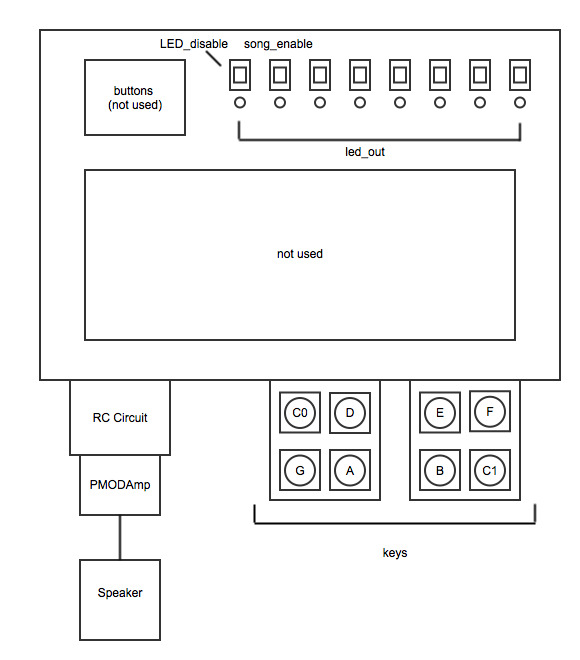
\includegraphics[width=2.75in]{img/FPGAtop.jpg}

    \end{multicols}

    The picture shown below displays the datapath and control of the circuit. The controller (a finite state machine) takes in all of the inputs and outputs the LEDs. It emits a signal corresponding to the note that needs to be output (a copy of the LED output) which is the Phase Accumulator receives. The data from the Phase Accumulator transfers to the Sine LUT, which goes to the Pulse Width Modulator... 

    For more information on how the circuit works, see section 2.3 ``Theory of Operation.''

    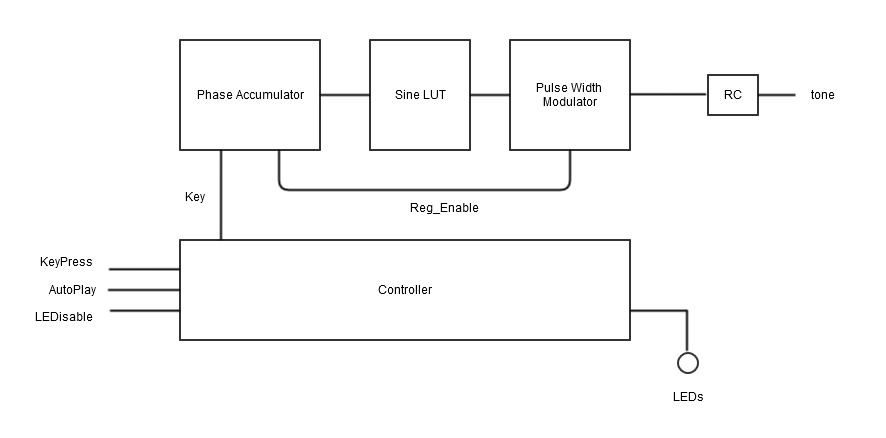
\includegraphics[width=5.5in]{img/basicblock.jpg}


  \subsection{Operating Instructions}

    % Operating instructions: Provide any information needed to set up and run your circuit. This is the User’s Manual part of your report.

    \begin{description}
      \item[Set up Circuit] \hfill \\
        To set up the one-octave keyboard circuit, you will need:
        \begin{itemize}
          \item Xilinx ISE Design Suite 14.4
          \item Digilent Adept
          \item The source code or the programming file
          \item 1 x Digilent NEXYS 3 Spartan 6 FPGA
          \item 2 x 4 button Digilent Button Module
          \item 1 x Digilent PmodBB
          \item 1 x Digilent PmodAMP2
          \item 1 x Speaker
        \end{itemize}

        Here are the steps to get the circuit running:
        \begin{enumerate}
          \item (If no bit file) Open the project in Xilinx, generate the programming file.
          \item Plug in FPGA (NEXYS 3 Spartan 6) into computer.
          \item Insert Digilent Button Modules in the top of JA1 and the top of JB1 on the NEXYS 3.
          \item Insert the Digilent PmodBB into JD1.
          \item Insert the PmodAMP2 into the top of J4 on the PmodBB. 
          \item Connect the speaker to J2 on PmodAMP2.
          \item Set up the RC circuit on the PmodBB.
          \item Open Digilent Adept, select bit file to program the FPGA.
        \end{enumerate}

      \item[Playing notes] \hfill \\
        To play notes, press the buttons on the FPGA corresponding to the notes that you want to play. There are two rows of four buttons. The top four buttons represent low c, d, e and f, while the bottom four buttons are g, a, b and high c.

        Only one note can be played at a time (first note pressed takes priority), and user-inputted notes only play when the auto-play switch is off.

      \item[Auto-play ``Kids'' by MGMT] \hfill \\
        To play ``Kids'' by MGMT, simply flip the AutoPlay switch on. You cannot create additional notes at this time using the buttons.

      \item[Disable LEDs] \hfill \\
        To disable the LEDs that light up corresponding to the notes that are pressed, simply turn on the LED disable switch.
        
    \end{description}

  \subsection{Theory of Operation}
  
    % Theory of operation: Discuss in detail how your circuit works. Start with a high-level overview of your design, illustrated by the block diagram. Give a prose description of each of the blocks and the interfaces between them. Describe what each block does and how it works. Make sure you discuss any tricks or functions that are not obvious from the logic diagram (e.g., ROMs used as lookup tables). From the information given in this section (with references to additional diagrams in the appendices), we should be able to reconstruct your design.

    The key component of our keyboard project is the geneneration of sine waves of varying frequencies using a technique called direct digital synthesis (DDS). To implement this, we use a combination of a phase accumulator and a sine wave lookup table (LUT) to produce wave samples of specific frequencies. In the place of a digital-to-analog converter, we use a pulse width modulator (PWM) to convert these sine wave samples to audio.

    % DANIEL ADD MORE ABOUT THE CONTROLLER
    8 different buttons (button module extensions on the FPGA), or ``key'' serve as the main ``playable'' interface of the keyboard. In VHDL, the keys are represented as an 8-bit bus input to the controller, where each bit represents a different note. Because our keyboard is monophonic, the controller checks each bit in succession from low to high C and outputs the first note it detects to the FreqLUT. As a result, only one bit in the 8-bit key_out vector received by ToneFreq-LUT should be high at a time; otherwise, when no button is being pressed, all bits are `0'. This prevents conflicts when multiple buttons are pressed at once. The controller also takes in an LED_disable input that disables the LEDs and a song_enable that automatically plays back a pre-programmed song (here ``Kids'' by MGMT).

    Key_out is then used as an index of sorts into the ToneFreq-LUT, which contains the pre-calculated phase increment values for each note, which is related to the desired frequency in the following way
        %equation increment = fdesired * 2^N/fclk
    where N represents the bit size of the accumulator and fclk is the frequency of the clock. We use N=13 here. This increment value is then passed on to the phase accumulator.

    The phase accumulator is essentially an incrementer composed of an adder and a register which increases by the increment value every clock cycle. However, although the system is running at a frequency of about 50MHz in order to reduce noise, in actuality the phase accumulator is updating at a frequency of around 10kHz, at the clk10 signal given by the PWMCounter. As a result, clk10 here serves as an enable.

  \subsection{Construction and Debugging}

    % Construction and debugging: Describe how you built and debugged your circuit. Which components did you build first? How did you test them? What problems did you have?

    To build the circuit, we began by building and testing the DDS and PWM. The

\section{Evaluation of Design}
  
  % Justification and evaluation of your design: Why is your solution better or worse than some reasonable alternatives? What might you do differently if you had it to do over again?

  Our solution is 

\section{Conclusions and Recommendations}

  % Conclusions: Summarize the goals and accomplishments of your project. Give a comparison of your original proposal (and final specifications) and the degree to which you achieved your proposed objectives. What recommendations do you have for future groups considering such a project? What words of general advice would you give to future groups?

  The original goal of our project was to simply make a one-octave keyboard that plays all the notes in C major. LEDs would light up when notes were played, unless an ``LED disable'' switch was turned on.

  At the end, we were not only able to accomplish our original goal of the simple keyboard but also to add an additional autoplay feature that played ``Kids'' by MGMT.

  For future groups looking to create this project, we would recommend that they really take the time to understand the operation of the circuit before jumping into the project. Another important consideration is to remember to synchronize the inputs and debounce the buttons throughout the project's creation.

\newpage
\section{Acknowledgments}

  % Acknowledgments: Technical reports and papers often have an acknowledgments section that thanks people other than the authors for their contributions. Use this section (if you wish) to acknowledge various sources (e.g. course staff, students, faculty, or others) for design ideas and other assistance.
  
  % In addition, you should use this section to explain the contributions of each partner to the project. (This is required.) For example, if each project partner was responsible for designing a different block of the system, state that here. If one partner had more responsibility for design, another for debugging, etc., describe that in this section. If different partners were responsible for different parts of the report, note that here.

  We would like to thank Eric Hansen and Dave Picard for their support and mentorship throughout not only this project but also the course. We would also like to thank the other students of Digital Electronics as well as the TAs. We'd also like to thank MGMT for an awesome song that conveniently contains itself to a single octave.

  5.1 and 5.2 list the contributions for each partner. Although both partners had their hands in most aspects of the project, some components generally had one partner who was more involved in its creation.

  \subsection{Vivian's Contributions}
    \begin{itemize}
      \item Circuit Design
      \item DDS, PWM, FreqLUT, PlayCount
      \item RC Circuit
      \item Block Diagrams
    \end{itemize}

  \subsection{Daniel's Contributions}
    \begin{itemize}
      \item Majority of the controller, including auto-play
      \item Design and creation of song auto-play, state diagram
      \item Top level
      \item Diagrams
      \item LaTeX for report
      \item Git creation/management
    \end{itemize}

\newpage
\section{References}

  % References: Cite any references (books, application notes) used in your design (e.g., for some clever circuit design). It is not necessary to acknowledge parts specifications (data sheets), unless you are quoting.

  \begin{thebibliography}{9}

  \bibitem{DDScordesses}
  	Cordesses, Lionel.
  	``Direct Digital Synthesis: A Tool for Periodic Wave Generation.''
  	\emph{IEEE Signal Processing Magazine.}
  	IEEE,
  	July 2004. 
  	Web.  	

  \bibitem{ENGS128Lab}
  	Hansen, Eric.
  	\emph{Lab Assignment 1.}
  	N.p.:
  	ENGS128 - Advanced Digital System Design, Spring 2011.
  	PDF.

  \bibitem{IntelDDS}
  	\emph{Introduction to Direct Digital Synthesis.}
  	San Jose: Intel Corporation,
  	June 1991.
  	PDF.

  \bibitem{MicrochipPWM}
  	Palacheria, Amar.
  	\emph{Using PWM to Generate Analog Output.}
  	N.p.: Microchip Technology Inc.,
  	1997.
  	PDF.

  \end{thebibliography}

\newpage
\section{Appendix}
  \listoffigures
  % Appendices: All the diagrams, etc, you collected go here.

  \newpage
  \subsection{System level diagrams}

    \subsubsection{Front Panel}
      
      % Front panel: An annotated digital photo of your project (Nexys2 board + add-ons) is helpful to show how you use the buttons, switches, LEDs, etc, and also where PMods plug in, etc.  

      \begin{figure}[H]
        \centering
        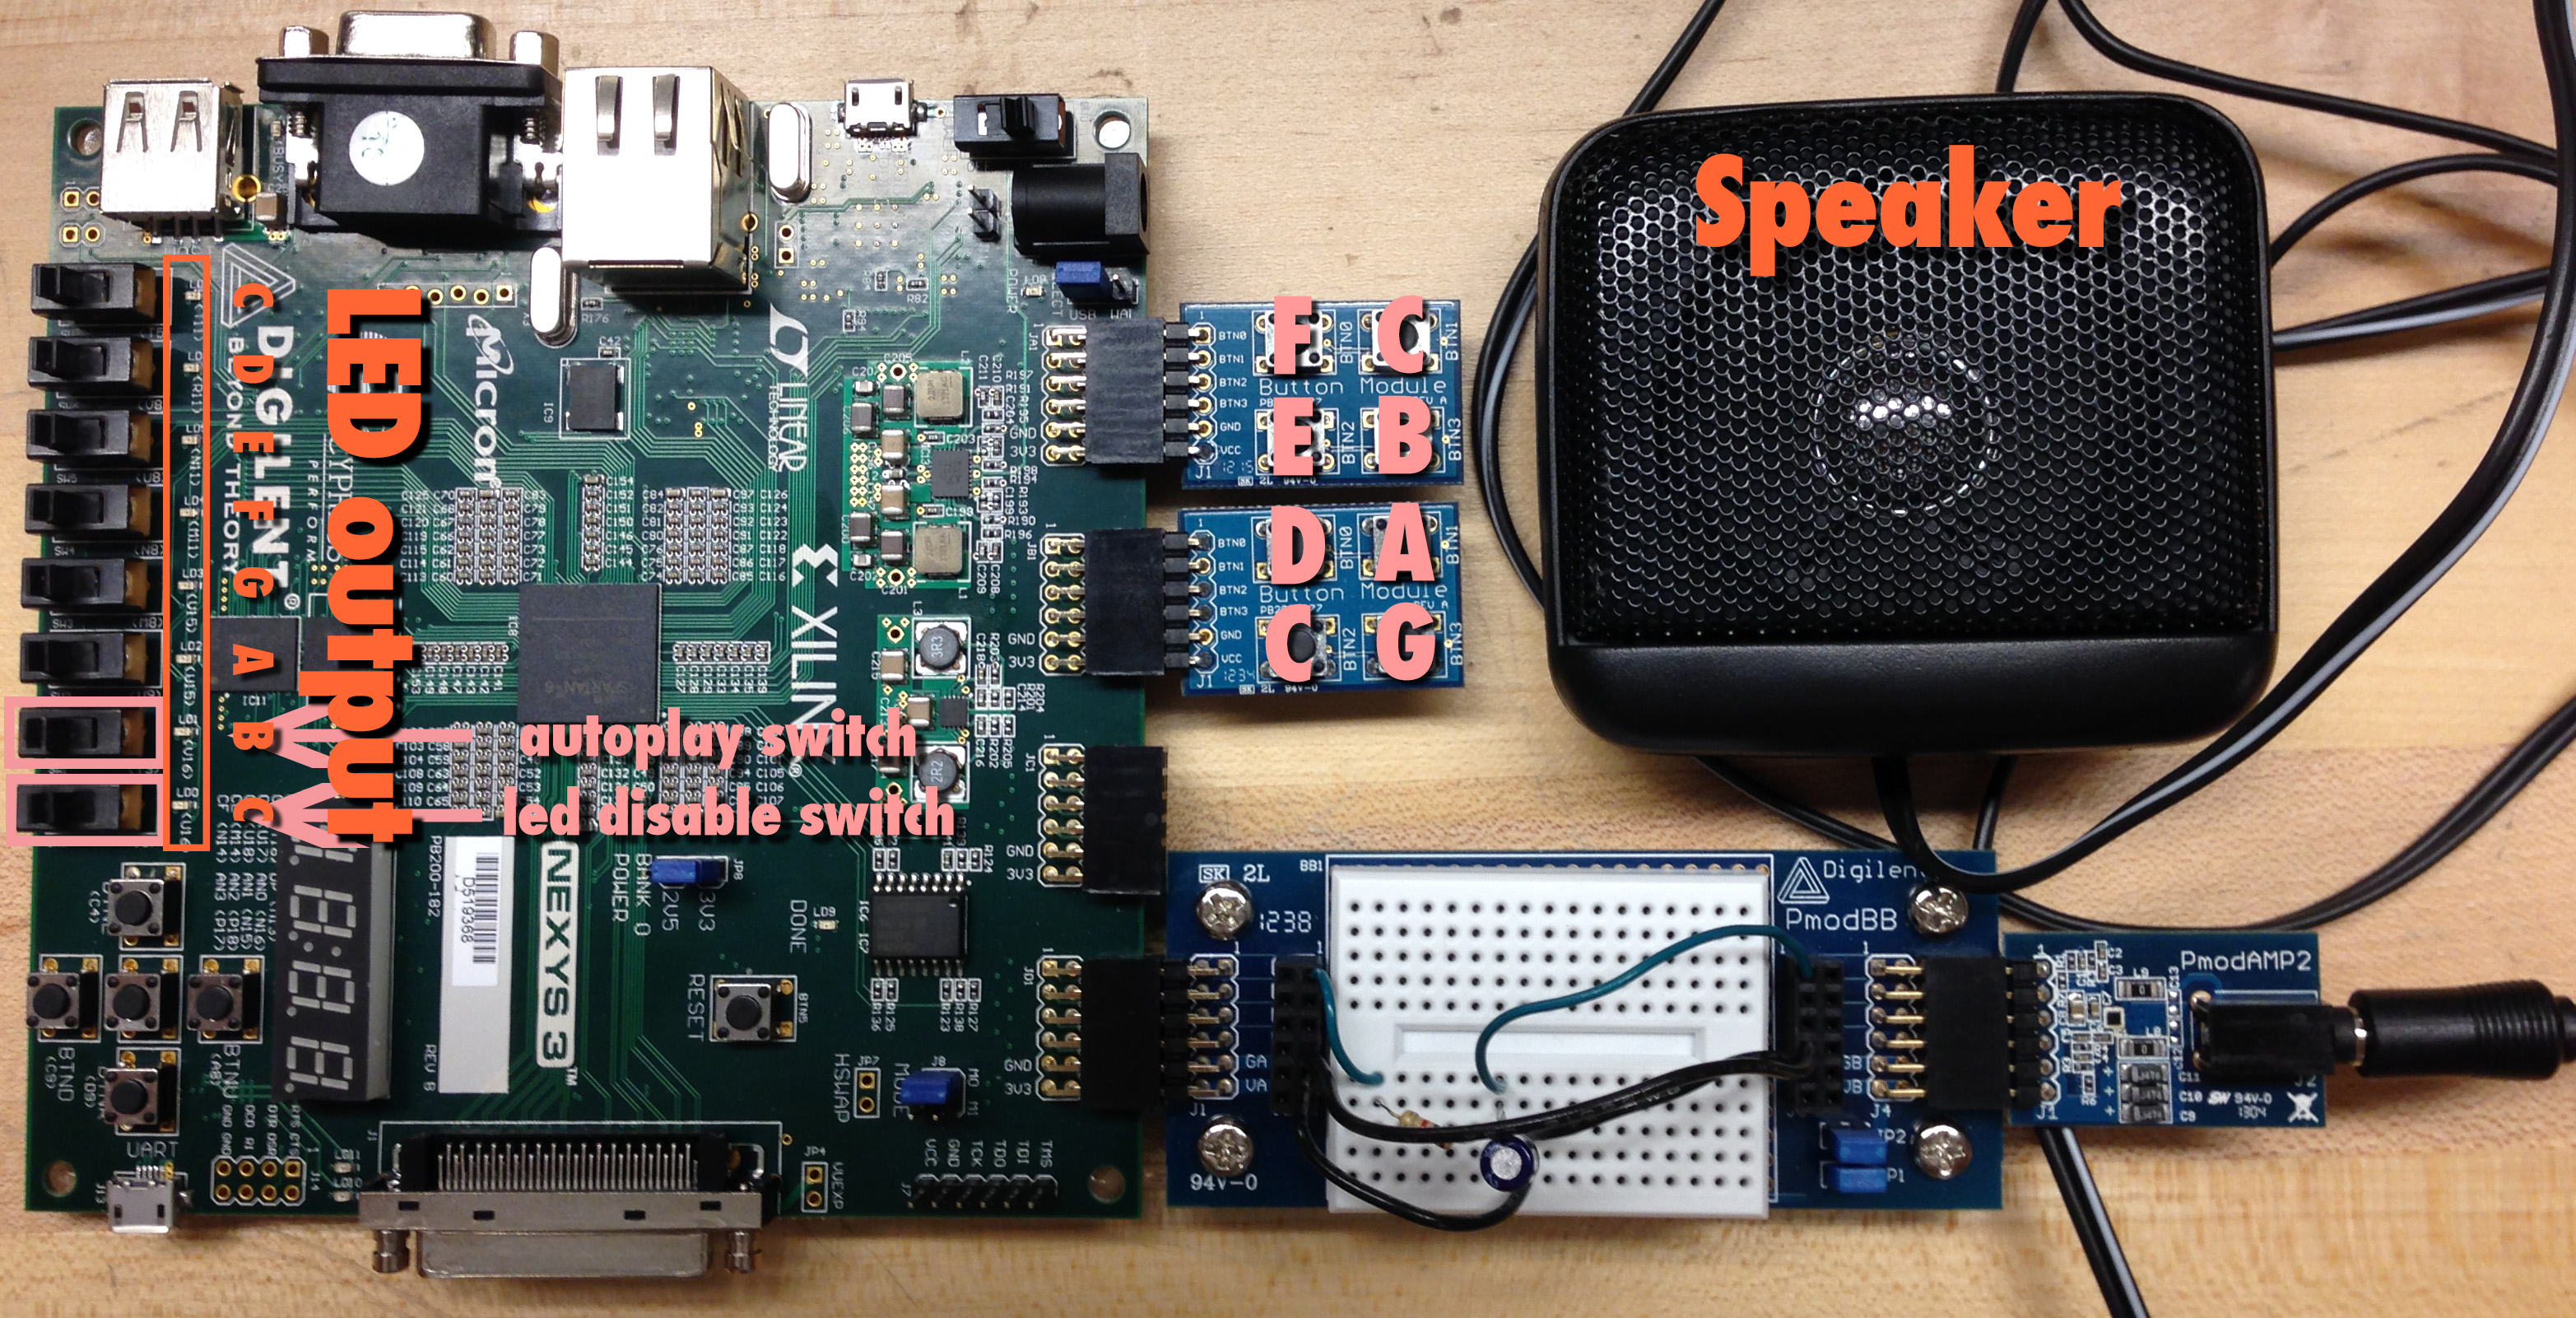
\includegraphics[width=6.5in]{img/annotated.jpg}
        \caption{Annotated Digital Photo of Project}
      \end{figure}

    \subsubsection{Block Diagram}
      % A functional block diagram which gives an overview of the hardware functional modules. By looking at this diagram, anyone else who has had the course should be able to understand what your project does. It is not necessary to use a drawing program to create your block diagram. A piece of graph paper and a ruler work just fine.

      % Each block, each input / output port in a block, and each net connecting blocks should be labeled with a descriptive name. Input ports for a drawing are always at the left edge of the drawing, and output ports are at the right edge. Additionally, ports that connect to/from Pmods or the FX2 breadboard must be labeled with a connector and pin number, e.g., JA-2 for pin 2 of the JA Pmod connector.
      % Here is a suggested hierarchy for your block diagrams:
      %   (1) The top level that shows the main functional blocks, including switches, displays, etc. At this level, the logic in your FPGA can be one big “black box” with ports labeled to match the port declarations in the top level of your logic design (whether VHDL or schematic).
      %   (2) The top level of logic in your FPGA. It’s simple to base your drawing on the RTL schematic generated by the Xilinx tool. If necessary, annotate it by hand so the reader can easily see what each block does.
      %   (3) Work down “recursively” into each block. Make sure your drawings are labeled in such a way that their place in the hierarchy is clear.

    \subsubsection{Schematic Diagram}
      % A schematic diagram with signal names and pin numbers for any off-board circuitry that you designed and built (i.e., on the FX2 board). The purpose of this diagram is to show how your project is wired up and to help in debugging if it doesn’t work. Make sure you include detailed schematic diagrams for any special circuits (e.g. LED arrays). Each package should be given a unique identifier, known as the reference designator: Un for integrated circuits (where n = 1, 2, ...), Rn for resistors, Cn for capacitors, Qn for transistors, Sn for switches, Pn and Jn for plugs and jacks, respectively, Dn for diodes. LEDn is sometimes used for LEDs or arrays of LEDs (like 7- segment displays). If you have other parts, ask me.% 

    \subsubsection{Package Map}
      % A package map showing where each component is located on your board. This only applies to off-board circuits that you built. The package map should resemble an "aerial photograph" showing clearly all connectors (labeled Jn or Pn), sockets, ICs (Un), switches (Sn), displays, etc. The package map is used as an intermediate stage between the logic diagram and your circuit.

      % Suppose you are troubleshooting your project. By studying the symptoms and your logic diagram, you deduce that there may be a wiring error at a particular part, e.g., a keypad encoder. On the logic diagram, that chip is labeled U8. You find U8 on the package map and it shows you precisely where to look on your circuit board to find the suspicious part. An easy way to create a package map is to annotate a digital photo of the board.

    \subsubsection{External Components}
      % Parts list: List all external components, including Pmods and parts that you wired up on the FX2 board. You don’t need a parts list if everything is confined to the Nexys board. Use sensible groupings (IC’s, discrete components, switches, connectors, etc.), and keep this list compact but complete. Omit trivial details like wire and wirewrap sockets.

      \begin{itemize}
        \item Design of
        \item The second item
        \item The third etc 
      \end{itemize}

    \newpage
	\subsection{Programmed Logic}

	    \subsubsection{State Diagrams}
	    	% for all state machines

		    
		    \begin{multicols}{2}
	    		For simplicity, the state machine for this program is represented in two state diagrams. The first, ``User Play State Diagram,'' represents the state machine for when the user is given input through the buttons. The second, ``Autoplay State Diagram,'' represents the state machine when the autoplay mode is on. Both state diagrams share an idle state. If the song enable switch if off, the ``User Play State Diagram'' should be used. If it is turned on, the ``Autoplay State Diagram'' should be used.

	    		The program starts at the idle state in the ``User Play State Diagram.'' If the song enable switch is turned on, the state jumps to autoidle in the ``Autoplay State Diagram.'' Otherwise, the state changes depending on the user's input.

		    \columnbreak

			    \begin{figure}[H]
			      \centering
			      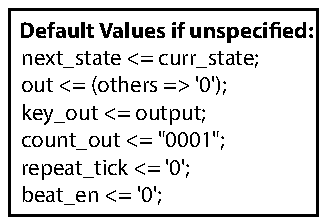
\includegraphics[width=2in]{img/StateDiagramDefaults}
			      \caption{State Diagram Defaults}
			    \end{figure}
		    \end{multicols}


	    
	      \begin{figure}[H]
	        \centering
	        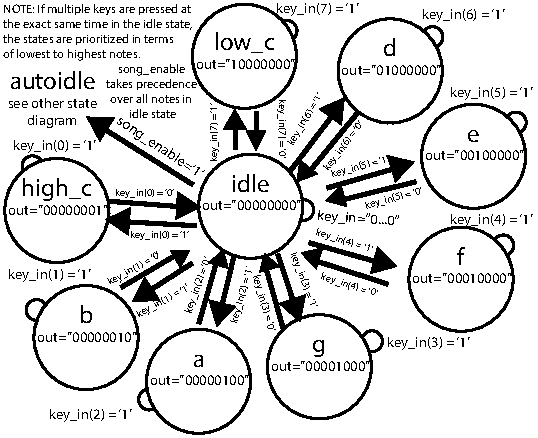
\includegraphics[width=6in]{img/UserStateDiagram}
	        \caption{User Play State Diagram}
	      \end{figure}
	      \newpage
	      \begin{figure}[H]
	        \centering
	        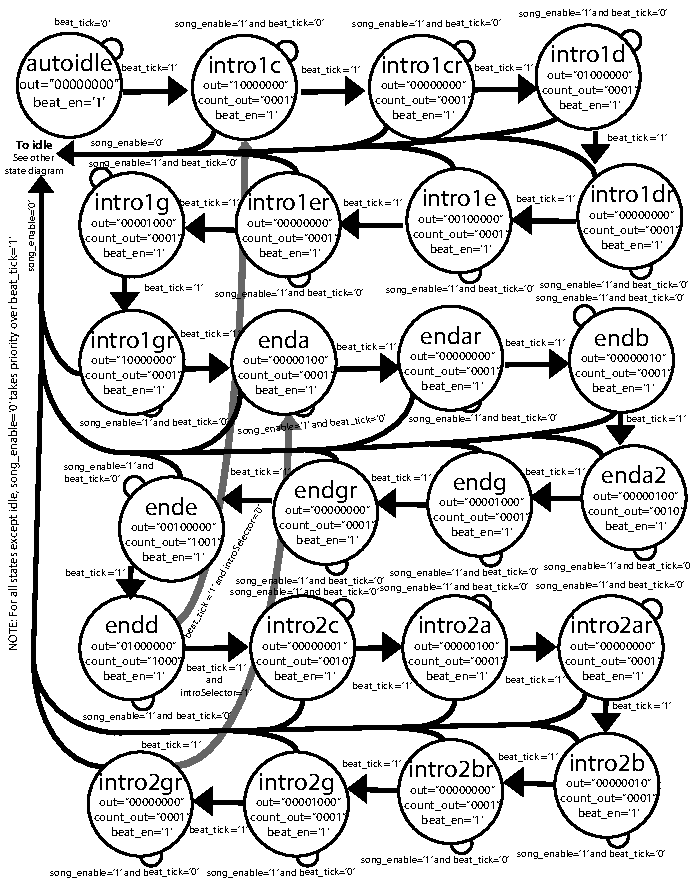
\includegraphics[width=6.5in]{img/AutoplayStateDiagram}
	        \caption{Autoplay State Diagram}
	      \end{figure}

	    \subsubsection{VHDL Code}
	      % for each module
	      Header comments removed.

	      \begin{figure}[H]
	        \caption{VHDL for Controller}
	        \begin{minted}{vhdl}
	  process
	  begin
	    CLK <= '1'; wait for 10 NS;
	    CLK <= '0'; wait for 10 NS;
	  end process;
	        \end{minted}
	      \end{figure}

	      \begin{figure}[H]
	        \caption{VHDL for DDS}
	        \begin{minted}{vhdl}
	library IEEE;
	use IEEE.STD_LOGIC_1164.ALL;
	use IEEE.NUMERIC_STD.ALL;

	entity DDS is
	   Generic (  ACCUMSIZE : integer := 13;
	          INDEXSIZE : integer := 8;
	          CLKFREQ     : integer := 100000000);
	          
	    Port (  clk     : in  STD_LOGIC;
	        step    : in  STD_LOGIC_VECTOR(ACCUMSIZE-1 downto 0);
	        clk10   : in  STD_LOGIC;
	        phase   : out STD_LOGIC_VECTOR(INDEXSIZE-1 downto 0));
	end DDS;

	architecture Behavioral of DDS is
	  signal curr_phase : unsigned(ACCUMSIZE-1 downto 0) := (others => '0');
	begin

	  AccumPhase: process(clk, clk10)
	  begin
	    if (rising_edge(clk)) then      
	      if (clk10 = '1') then     
	        curr_phase <= curr_phase + unsigned(step);
	      end if;
	    end if;
	  end process AccumPhase;
	  
	  phase <= std_logic_vector(curr_phase(ACCUMSIZE-1 downto ACCUMSIZE-INDEXSIZE));
	end Behavioral;
	        \end{minted}
	      \end{figure}

	      \begin{figure}[H]
	        \caption{VHDL for PWM}
	        \begin{minted}{vhdl}
	  process
	  begin
	    CLK <= '1'; wait for 10 NS;
	    CLK <= '0'; wait for 10 NS;
	  end process;
	        \end{minted}
	      \end{figure}

	      \begin{figure}[H]
	        \caption{VHDL for PlayCount}
	        \begin{minted}{vhdl}
	  process
	  begin
	    CLK <= '1'; wait for 10 NS;
	    CLK <= '0'; wait for 10 NS;
	  end process;
	        \end{minted}
	      \end{figure}

	      \begin{figure}[H]
	        \caption{VHDL for FreqLUT}
	        \begin{minted}{vhdl}
	library IEEE;
	use IEEE.STD_LOGIC_1164.ALL;
	use IEEE.NUMERIC_STD.ALL;

	entity FreqLUT is
	   Generic (  ACCUMSIZE : integer := 13;
	          CLKFREQ     : integer := 10000);
	          
	    Port ( clk : in  STD_LOGIC;
	           key_in : in  STD_LOGIC_VECTOR (7 downto 0);
	           increment : out  STD_LOGIC_VECTOR (ACCUMSIZE-1 downto 0));
	end FreqLUT;

	architecture Behavioral of FreqLUT is
	  constant PHASECONSTANT : integer := 2**ACCUMSIZE;
	  constant LOWC : integer := 262;
	  constant D : integer := 294;
	  constant E : integer := 330;
	  constant F : integer := 349;
	  constant G : integer := 392;
	  constant A : integer := 440;
	  constant B : integer := 494;
	  constant HIGHC : integer := 523;
	begin

	  getIncrement: process(key_in)
	  begin
	  
	    if (key_in(7) = '1') then
	      increment <= std_logic_vector(to_unsigned(LOWC * PHASECONSTANT / CLKFREQ, ACCUMSIZE));
	    elsif (key_in(6) = '1') then
	      increment <= std_logic_vector(to_unsigned(D * PHASECONSTANT / CLKFREQ, ACCUMSIZE));
	    elsif (key_in(5) = '1') then
	      increment <= std_logic_vector(to_unsigned(E * PHASECONSTANT / CLKFREQ, ACCUMSIZE));
	    elsif (key_in(4) = '1') then
	      increment <= std_logic_vector(to_unsigned(F * PHASECONSTANT / CLKFREQ, ACCUMSIZE));
	    elsif (key_in(3) = '1') then
	      increment <= std_logic_vector(to_unsigned(G * PHASECONSTANT / CLKFREQ, ACCUMSIZE));
	    elsif (key_in(2) = '1') then
	      increment <= std_logic_vector(to_unsigned(A * PHASECONSTANT / CLKFREQ, ACCUMSIZE));
	    elsif (key_in(1) = '1') then
	      increment <= std_logic_vector(to_unsigned(B * PHASECONSTANT / CLKFREQ, ACCUMSIZE));
	    elsif (key_in(0) = '1') then
	      increment <= std_logic_vector(to_unsigned(HIGHC * PHASECONSTANT / CLKFREQ, ACCUMSIZE));
	    else 
	      increment <= (others => '0');
	    end if;
	  
	  end process getIncrement;
	end Behavioral;
	        \end{minted}
	      \end{figure}

	    \subsubsection{Resource utilization}
			\begin{figure}[H]  
				\caption{Advanced HDL Synthesis Report}
	   			\begin{lstlisting}
Macro Statistics
# Counters                                             : 3
 14-bit up counter                                     : 1
 32-bit up counter                                     : 1
 4-bit up counter                                      : 1
# Accumulators                                         : 1
 13-bit up accumulator                                 : 1
# Registers                                            : 8
 Flip-Flops                                            : 8
# Comparators                                          : 2
 10-bit comparator greater                             : 1
 4-bit comparator equal                                : 1
# Multiplexers                                         : 10
 1-bit 2-to-1 multiplexer                              : 2
 13-bit 2-to-1 multiplexer                             : 7
 8-bit 2-to-1 multiplexer                              : 1
# FSMs                                                 : 1
	   			\end{lstlisting}
	   		\end{figure}

	   		\begin{figure}[H]  
	   			\caption{Device Utilization Summary}
	   			\begin{lstlisting}
Slice Logic Utilization: 
 Number of Slice Registers:             189  out of  18224     1%  
 Number of Slice LUTs:                  335  out of   9112     3%  
    Number used as Logic:               335  out of   9112     3%  

Slice Logic Distribution: 
 Number of LUT Flip Flop pairs used:    346
   Number with an unused Flip Flop:     157  out of    346    45%  
   Number with an unused LUT:            11  out of    346     3%  
   Number of fully used LUT-FF pairs:   178  out of    346    51%  
   Number of unique control sets:        20

IO Utilization: 
 Number of IOs:                          29
 Number of bonded IOBs:                  29  out of    232    12%  
    IOB Flip Flops/Latches:               2

Specific Feature Utilization:
 Number of BUFG/BUFGCTRLs:                2  out of     16    12%  
	   			\end{lstlisting}
	   		\end{figure}


  \subsection{Memory Map}
    % Memory map: If you are using a memory chip or block memory in the FPGA as a complex look-up table or for data storage, show how the address and data bit patterns are partitioned among the logical variables involved (e.g., for storing sound clips, address bits 12-13 are which sound, and address bits 0- 11 are samples within a sound).



  \subsection{Timing Diagram}
    % A timing diagram, e.g., generated from a behavioral simulation, showing all important signals. It is not necessary to duplicate timing diagrams which may be found in a data sheet or user’s manual (e.g., for memory chips).


  % ADDITIONAL SUBSECTIONS?
  % 6. Copies of data sheets for any special components you used that aren’t already on the class website.
  % 7. Computer programs (e.g., Matlab codes used to generate lookup tables, etc).
  % 8. Other documentation. Include anything else that might be needed to understand or reproduce your design.


\end{document}


